\documentclass{report}

\usepackage[utf8]{inputenc}
\usepackage{textgreek}
\usepackage{blindtext}
\usepackage[inference]{semantic}
\usepackage{multicol}
\usepackage{hyperref}
\usepackage[newfloat]{minted}
\usepackage{amssymb}
\usepackage{amsmath}
\usepackage{graphicx}
\usepackage{svg}
\usepackage[capitalise]{cleveref}
\usepackage{enumitem}
\usepackage{float}
\usepackage{microtype}
\usepackage[a4paper, margin=1in]{geometry}
\usepackage{fancyvrb, newverbs, xcolor}
\usepackage{caption}
\usepackage[UKenglish]{babel}
\usepackage[parfill]{parskip}

\definecolor{cverbbg}{gray}{0.93}
\newcommand{\vtilde}{$\sim\ $}

\newenvironment{equ}{\vspace{0mm}\captionsetup{type=listing}}{\vspace{2mm}}
\SetupFloatingEnvironment{listing}{name=Code Snippet}

\newcommand{\spipe}{\quad\lvert\quad}
\newcommand{\ctexttt}[1]{\colorbox{cverbbg}{\texttt{#1}}}
\newverbcommand{\cverb}
  {\setbox\verbbox\hbox\bgroup}
  {\egroup\colorbox{cverbbg}{\box\verbbox}}

\hypersetup{
    colorlinks = true,
    urlcolor = blue,
    linkcolor = blue,
    citecolor = red
}

\newcommand\MyBox[1]{
  \fbox{\lower0.75cm
    \vbox to 1.7cm{\vfil
      \hbox to 1.7cm{\hfil\parbox{1.4cm}{#1}\hfil}
      \vfil}%
  }%
}

\newcommand{\hs}{\mintinline{haskell}}
\newcommand{\mono}{\mintinline{text}}

\begin{document}

%Start of titlepage!
\begin{titlepage}
    \centering
    
    \textls{\textsc{\huge{Utrecht University}}}\\
    \vspace{5em}
    \textsc{\Large{Thesis Report}}\\
    \vspace{2em}
    \textsc{\large{Department of Information and Computing Sciences}}\\
    
    \vspace{3em}
    \hrulefill
    \vspace{4em}
    
    \huge{Embracing Core \& Supervising the Optimisation Pipeline}\\
    \vspace{1em}
    \Large{Empowering Haskell developers with a looking glass into the core2core pipeline}

    \vspace{4em}
    \hrulefill
    \vspace{3em}
   
    \begin{tabular}{p{0.5\textwidth}r}
        \textit{Author:} & \textit{Supervisors:}\\
        H.A. Peters, BSc & W. Swierstra\\
        h.a.peters@uu.nl & T. McDonall\\
        5917727 &
    \end{tabular}
    
    \vspace{3em}
    \textsc{December 2022}\\
    % \textsc{\textcolor{red}{Version: Draft 2}}
    
    \begin{figure}[b]
        \hspace{-1.25cm}
        \includegraphics{figs/UU_logo_2021_NL_RGB.png}
    \end{figure}
    
\end{titlepage}

\vspace*{\fill}
\begin{center}
\begin{minipage}{.7\textwidth}
\centerline{\textbf{Abstract}}
Straight away communicate the idea that core exploration should be easier and more approachable and give
and drill it home with a small but daunting core snippet.
 
Haskell is a language explicit about side effects which allows for pretty drastic semantic preserving transformations,
inviting programmers to hand over a lot of optimisation responsibilities. To reasure success one needs to explore
interactions with the compiler.


\end{minipage}
\end{center}
\vfill % equivalent to \vspace{\fill}

\thispagestyle{empty}

\newpage
\clearpage
\pagenumbering{roman}
\tableofcontents

\newpage
\clearpage
\pagenumbering{arabic}

%Add with newpage
\newpage

\chapter{Introduction}

\section{GHC, an optimising compiler}

\subsection{Write good code not fast code}
Haskell is a high level language designed to write highly composable functions.
This leads to a juxtaposition where programmers are encouraged to write code that
is not necessarily fast to evaluate. An extremely common example is the composition
of list operations. Consider the function \mono{halves} which divides each element
in a list of \mono{Int}s, discarding those that are not a multiple of 2.

\begin{listing}[H]
\begin{minted}[linenos]{haskell}
halves :: [Int] -> [Int]
halves = map (`div` 2) . filter even
\end{minted}
\end{listing}

Both \mono{map} and \mono{filter} are defined as a loop over a list, constructing a new one. 
If \mono{halves} were to be compiled as is, it would produce two loops as well as allocating
an intermediate list. Of course, it would be possible to rewrite the function to circumvent this
issue:

\begin{listing}[H]
\begin{minted}[linenos]{haskell}
halves_fast :: [Int] -> [Int]
halves_fast [] = []
halves_fast (x:xs) = 
  let 
    tl = halves_fast xs 
  in if even x 
     then (x `div` 2):tl
     else tl
\end{minted}
\end{listing}

But requiring the programmer to do such rewrites manually tragically undermines
the virtue of compositional style programming. Code simply would be harder to read, write,
and maintain and consequently tend to be less correct. 

Luckily, GHC does address this issue - and many others - with an extensive set of optimisation transformations.
This particular program will benefit greatly from the fusion system which specifically deals with removing
the intermediate lists. This a well-established optimisation that is also referred to as deforestation. \cite{WADLER1990231}

As a result, compiling with these optimisations enabled will result in a syntactically equivalent
definition for \mono{halves} and \mono{halves_fast}.

\subsection{The cascade effect}

Optimisation transformations are applied is a certain order, giving rise to the \textit{cascade effect}. \cite{haskell_optimisations_1997}
This effect refers to the dramatic consequences that the order of transformations can have. 

Let us study another example that showcases a problematic tug-of-war between in-lining functions
and applying rewrite rules. In-lining is very common optimisation that simply replaces variables
with their definition. This reduces the need to allocate thunks for let bound variables as well as 

A commonly encountered situation where the cascade effect comes into play,
is the tug-of-war between in-lining functions (replacing a function call with its RHS) and applying rewrite rules. Consider
the following example of a binary tree,  a function to that facilitates mapping over each \hs{Leaf}, as well a function
that composes two integer additions over the tree.

\begin{minted}[linenos]{haskell}
module Tree where

data Tree a = Leaf a | Node (Tree a) (Tree a) deriving Show

mapTree :: (a -> b) -> Tree a -> Tree b
mapTree f (Leaf x) = Leaf (f x)
mapTree f (Node lhs rhs) = Node (mapTree f lhs) (mapTree f rhs)

addFive :: Tree Int -> Tree Int
addFive = mapTree (+1) . mapTree (+4)
\end{minted}

The \mono{addFive} function is implemented non-optimally; by traversing
over the tree structure twice, an intermediate structure will be allocated
and the structure will have to be traversed twice.

To combat this issue, we could add the rewrite rule \textit{mapTree/mapTree}:
\begin{minted}[linenos]{haskell}
{-# Rules
   "mapTree/mapTree"   forall f g.   mapTree f . mapTree g    = mapTree (f. g)   ;
#-}
\end{minted}

This rule informs GHC of the ability to \textit{fuse} a subsequent tree mapping.
This rules is considered a form of \textit{deforestation}: 
The elimination of intermediate structures \cite{WADLER1990231}.

Sadly however, the effort was in vain: the rule never fired! The reason - as was
foreshadowed - is interference with the in-liner. Before our rule is considered, \mono{addFive}
is transformed by eta expanding and in-lining \mono{(.)} which produces: 

\begin{minted}{haskell}
addFive :: Tree Int -> Tree Int
addFive x = mapTree (+1) (mapTree (+4) x)
\end{minted}

But this no longer syntactically matches the LHS of our \mono{mapTree/mapTree} rule. What we have thus shown
is that we could improve the optimisation pipeline in this specific case by considering our
rewrite rule before we inline a function. On contrary, it does not take much imagination to
realise that there will be many other programs for which the opposite holds.

The important point is that one optimisation may open or close the door to many other
optimisations down the road. It thus becomes clear that the interaction of a Haskell program
with the optimiser may be quite unstable and consequently sensitive to small changes. 
Changes not only in the source but also in the build environment (a minor release of
the compiler comes to mind). Thus, we cannot trust that our successfully optimised program will remain
optimised in the future. We observe that each program we write may require specific, manual, 
effort to be made more efficient.


\chapter{Research Questions}


\paragraph{Main Question} 
How can GHC’s core2core passes be captured and presented in such a way that core
inspection becomes a more successful, and easier task?

\hfill \break

\paragraph{Sub-Question 1} 
How does one efficiently navigate where small changes occur in two or more captures?

\paragraph{Sub-Question 2}
How to make viewing core more manageable using various display options?

\paragraph{Sub-Question 3}
How could performance regressions that have occurred in the past in popular Haskell projects,
have been resolved faster?

\chapter{Background}

\section{A Core Language}

GHC recognises three distinct stages of the compilation process. \cite{haskell_optimisations_1997}

% A latex list with frontend, middle, backend
\begin{enumerate}
  \item \textbf{Frontend}, parsing and type checking, enables to give clear errors that reference the unaltered source code.
  \item \textbf{Middle}, a number of optimisation transformations.
  \item \textbf{Backend}, generates and compiles to machine code, either via C-- or LLVM.
\end{enumerate}

The middle section is tasked with doing all the optimisation work it can, leaving only those optimisations to the backend
it can't otherwise perform. Within the middle section, the work is further split into sub-stages, where each transformation
is a separate, composable pass. An obvious benefit to this approach is that each pass can be tested independently. Moreover, because
the types are preserved throughout the middle section, it can be verified that each transformation does not violate the typesystem;
A strong bit of evidence towards the correctness of the compiler.

Regardless, the Haskell source language itself is not a good target for optimisation transformations. The source language wants
to be rich and expressive, which yields a datatype of over 100 constructors. Any transformation over such a datatype has far too
many cases to be considered practical to implement; Not to mention the myriad of bug-inducing edge cases. To overcome this issue, the
middle section first performs a desugaring pass, translating the source language into a far simpler intermediate language
called \textit{Core}. 

Core --- which is how we will refer to GHC intermediate representation going forward --- is designed to be as simple as possible
without being impractical. A testament to that property is the fact that we can fit the entire definition on the page:

\begin{listing}[H]
\begin{minted}{haskell}
data Expr
  | Var Id
  | Lit Literal
  | App Expr Expr
  | Lam Bndr Expr
  | Let Bind Expr
  | Case Expr Bndr Type [Alt]
  | Cast Expr CoercionR -- safe coercions are required for GADTs
  | Tick Tickish Expr  -- annotation that can contain some meta data
  | Type Type
  | Coercion Coercion
  
data Alt = Alt AltCon [Bndr] Expr
 
data Bind
  = NonRec Bndr Expr
  = Rec [(Bndr, Expr)]
  
-- the Var type contains information about
-- a variable, like it's name, a unique identifier
-- and analysis results
type Bndr = Id
type Id = Var

type Program = [Bind]
\end{minted}
\label{code:core_def}
\caption{An ever so slightly simplified version of the Core Language}
\end{listing}

Writing an optimisation transformation essentially of type \hs{Program \rightarrow Program} does not now seem
as daunting given the drastically reduced number of cases to consider. 
Likewise, maintaining and debugging transformations is much less of a strenuous task.

\section{The core2core transformations}

Over its numerous decades of development, the core2core pipeline has been fitted with a myriad of transformations.
It would be impractical to discuss all them here. However, we will discuss in depth the role of the four 5 simplifier
passes, as well as the worker/wrapper transformation. The first because it gives context to the rewrite rules and the latter
because it is a natural bridge to unboxed types; both concepts which will become relevant in discussing the results of this thesis.

\subsection{The simplifier: its parts}

The simplifier is quite literally an indispensable part of the transformation pipeline. Although the parts of the pipeline
are meant to be seperable entities, they heavily rely on the simplifier to deal with the cleanup. As such, it has earned
itself the reputation of being the workhorse of the pipeline. \cite{ghc_wiki}

If you were looking for an atom, you have not found it. The simplifier is in itself again a collection of smaller transformations,
albeit applied concurrently. Each simplifier subpart is a local transformation, that is, it only looks at the immediate
surroundings of the expression. We give a near comprehensive list of each subpart along with an example:

\subsubsection{Constant Folding}
Evaluate expressions that require no runtime information. This is a very logical transformation that does not
require any considerations.

\begin{listing}[H]
\begin{minted}{haskell}
-- before
3 + 4
-- after
7
\end{minted}
\end{listing}

\subsubsection{Inlining-1}

Inlining function calls is a well known performance enhancing operation in all language, but especially so in functional ones.
The difference is staggering with a around 10-15\% performance increase for conventional languages, as opposed to
30-40\% for functional languages. \cite{haskell_optimisations_1997} \cite{c_inliner}.

Unlike constant folding, it is not an ad-hoc no brainer. An easy case would be to inline a function that is
used exactly once. All that this does is remove the veil that hides the function body for further optimisations:

\begin{listing}[H]
\begin{minted}{haskell}
-- before
f x = x + 1
f 3
-- after
3 + 1
\end{minted}
\end{listing}

However, if the function is used in multiple locations with different arguments, you risk increasing the size of the program
because the function body will be duplicated at each call-site. This is a trade-off that --- altough often worth it --- must be
considered on a case to case basis. GHC has a number of heuristics to determine whether inlining is worth it or not. Obviously,
this cannot be a perfect solution and one can imagine how a small change in the code can suddenly cause the inliner to reverse
its decision; a testament to the non-continuous nature of the compiler.

\subsubsection{Inlining-2}

Let bindings are often described as syntax sugar for lambda abstractions, there is an important difference to be considered.
Because let bindings in Haskell are lazily evaluated, it may lead to explosion if the let bound variable is used in a lambda
expression. For example:

\begin{listing}[H]
\begin{minted}{haskell}
-- before, 'expensive' is called at most once
let v = expensive 42
    l x = ... v ...
in map xs

-- after, 'expensive' is called for each element of 'xs'
let l x = ... expensive 42 ...
in map xs
\end{minted}
\end{listing}

This transformation would be disastrous for performance and GHC will take greate care to avoid it. 

\subsubsection{Case of known constructor}

The case destruction is only the way to get to the WHNF of an expression. This means that inside of a case expression
we have learned information about the variable under scrutiny and can use it to infer the result of outer case expressions.
Consider the following scenario:

\begin{listing}[H]
\begin{minted}{haskell}
safe_tail :: [a] -> [a]
safe_tail list = case list of
  [] -> []
  x:xs -> tail list
\end{minted}
\end{listing}

Which inlining will transform into:

\begin{listing}[H]
\begin{minted}{haskell}
safe_tail :: [a] -> [a]
safe_tail list = case list of
  [] -> []
  x:xs -> case xs of
    [] -> error "tail of empty list"
    (x:xs) -> xs
\end{minted}
\end{listing}

Since we scrutinize \mono{xs} again in the inner case, we actually already know that the second case is only ever called,
thus we can eliminate the case expression as a whole.

\begin{listing}[H]
\begin{minted}{haskell}
safe_tail :: [a] -> [a]
safe_tail list = case list of
  [] -> []
  x:xs -> xs
\end{minted}
\end{listing}

The removal of the call \mono{error} is a testament to this function being deserving of the \mono{safe} prefix.

\subsubsection{Case of case}

There are cases (no pun intended) where the case-of-know-constructor cannot quite do its job, although it is obvious
that benefits are still to be gained. Consider for example what happens when instead of scrutinizing the same variable,
the outer case scrutinizes the result of the innner case:


\begin{listing}[H]
\begin{minted}{haskell}
-- before (possibly desugared from 'if (not x) then E1 else E2'
-- after also inlining 'not')
case (case x of {True -> False; False -> True}) of
  True -> E1
  False -> E2
\end{minted}
\end{listing}

We might hope to gain something from the information that the inner case has produced by moving the outer case expression
to each branch of the inner one:

\begin{listing}[H]
\begin{minted}{haskell}
case x of
  True -> case False of {True -> E1; False -> E2}
  False -> case True of {True -> E1; False -> E2}
\end{minted}
\end{listing}

Now we can rely on constant folding to simplify all the way down to:

\begin{listing}[H]
\begin{minted}{haskell}
case x of
  True -> E2
  False -> E1
\end{minted}
\end{listing}

Note that we do risk duplicating \mono{E1} and \mono{E2} if the expression does not reduce so completely.
A solution to this are \textit{join points}, which we will not go into here for the sake of brevity.

\subsubsection{Rewrite rules}

We already discussed in \cref{section:introduction:rewrite_rules} how rewrite rules are way to express domain
specific knowledge to the compiler that it otherwise can't practically infer. Applying given rewrite rules is task
also given to the simplifier. It should now be clear that this process can get a little messy since the simplifier
is under no obligation to apply the rules, nor its other tasks, in any particular order. We will get into this issue
more in the next section where we discuss the simplifier at large.

It should be noted that the use of rewrite rules are very common during the compilation of most any haskell program.
This is because the internal fusion system on list operations are implemented as built in rewrite rules.
We discuss this system more in depth in \cref{section:background:fusion}.



\subsection{The simplifier: its sum}

An attentive reader might have noticed that when explaining one part of the simplifier, we often relied on another to
its job. This begs the question: how does the simplifier determine in which order to run its subparts. The answer to that is
that it does not. The analogy here is that a compiler is a gun and a program is a target. Every program is very different
and we cannot know in advance how to best hit it. Therefore, we must ensure that the compiler --- or this case the simplifier stage ---
has a lot of bullets in its gun to ensure being able to effectively hit a lot of targets. \cite{haskell_optimisations_1997}

A secondary problem with this approach is that one simplifier part may enable another to its job after. Running the simplifier
once is therefore not satisfactory and we must run it until it reaches a sort of \textit{fixed point}. At least up until some
arbitrary limit since there is no guarantee such a fixed point exists and even if it does that we find it and not get stuck in a loop.

Aforementioned looping beheavior can actually occur quite easily due to certain rewrite rules. It is not always the case that
the RHS of a rewrite rules objectively better than the right. It might be that the rewrite is benificial because it \textbf{may}
enable other optimisation to take place afterwards. However, if for some reason that did not turn out to be possible, we may want
to apply the reverse rewrite rule later. This is obviously problematic as we can be ping-pong between rewrite rules forever.
To overcome that issue one can enable/disable rewrites rules in certain phases of simplifier. To understand this we must first
understand when the simplifier is run.

In order, the simplifier is --- rather unituitively --- interspersed between other transformations as follows:

\begin{enumerate}
  \item \textbf{Gentle} (disables case-of-case transformations)
  \item \textbf{Phase 2}
  \item \textbf{Phase 1}
  \item \textbf{Phase 0}
  \item \textbf{Final}
\end{enumerate}

By default, rewrite rules as well as inlinings can occur in each of these phases but the programmer does have to ability
to specify devations from this beheavior. For example, in the \mono{text} library, we find in the \mono{Data.Text} module
the following snippet:

\begin{listing}[H]
\begin{minted}{haskell}
-- This function gives the same answer as comparing against the result
-- of 'length', but can short circuit if the count of characters is
-- greater than the number, and hence be more efficient.
compareLength :: Text -> Int -> Ordering
compareLength t c = S.compareLengthI (stream t) c
{-# INLINE [1] compareLength #-}

{-# RULES
"TEXT compareN/length -> compareLength" [~1] forall t n.
    compare (length t) n = compareLength t n
#-}
\end{minted}
\end{listing}

Here phase control is used to indicate that \mono{compareLength} should \textbf{only} be inlined in phase 1 and conversely
that the rewrite rule \textbf{compareN/length} maybe applied \textbf{except} in phase 1. What this ensures is that the inliner
will not operate on the result of the rewrite rule directly in the same phase. This is supposedly because we expect \mono{compareLength}
to occur in the LHS of a different rewrite rule which is to be desired over inlining at first.

\subsection{The worker/wrapper transformation}

\section{The fusion system}
\label{section:background:fusion}

build/fold using rewrite rules

\section{Contemporary Haskell comprehension}

\subsection{Communicating in Core}
\label{section:communicating_core}

We are not pioneers discovering the land of Core inspection. Since its inception, Core has
been used to communicate about programs and compiler interactions. Sifting through open issues on the
GHC compiler itself, one quickly comes across discussions elaborated by Core snippets. Consider issue
\href{https://gitlab.haskell.org/ghc/ghc/-/issues/22207}{\#22207} titled `\textit{bytestring Builder performance regressions after 9.2.3}' for example.
\hfill \break

\textit{While testing the performance characteristics of a bytestring patch meant to mitigate withForeignPtr-related performance regressions,
it was noticed that several of our Builder-related benchmarks have also regressed seriously for unrelated reasons.
The worst offender is byteStringHex, which on my machine runs about 10 times slower and allocates 21 times as much when using ghc-9.2.4 or ghc-9.4.2
as it did when using ghc-9.2.3. Here's a small program that can demonstrate this slowdown:}
\hfill \break

It then provides two snippets containing the final Core representation of \mono{byteStringHex} as produced by the two different GHC version.
Each of these documents are around 400 lines of un-highlighted code with all available information. And while having all available information
sounds like a good thing (and it is in a way) it poses a serious practicality issue.
Namely: it is exceedingly difficult for a human to read and comprehend a certain aspect of the AST while having to filter out another.
Not to mention, it solidifies reading Core as an activity reserved for only the most expert Haskell developers by, scaring others away with
a steep barrier to entry.

\subsection{Current tooling}

\subsubsection{GHC itself}


Core snippets of your program can easily be coerced out of GHC. The most information you can get
is the Core AST at each pass of the optimisation pipeline by using \mono{-ddump-core2core}.
To reduce the signal-to-noise ratio of Core snippets, one can use any number of suppression options.
It is common to suppress type arguments and type applications for example. These are largely
uninteresting because Core is only typed to facilitate the correctness preserving checks that \mono{core-lint} performs
and do not affect the compilation in any way.

As can be read in the GHC documentation, the following suppression flags are available to help to tame the beast.

\begin{table}[H]
  \begin{tabular}{p{0.35\linewidth}|p{0.65\linewidth}}
  \textbf{GHC flag} & \textbf{Effect on core printing} \\
  \hline
           & \\
  \mono{-dsuppress-all} & In dumps, suppress everything (except for uniques) that is suppressible.  \\
  \mono{-dsuppress-coercions} & Suppress the printing of coercions in Core dumps to make them shorter  \\
  \mono{-dsuppress-core-sizes} & Suppress the printing of core size stats per binding (since 9.4)  \\
  \mono{-dsuppress-idinfo} & Suppress extended information about identifiers where they are bound  \\
  \mono{-dsuppress-module-prefixes} & Suppress the printing of module qualification prefixes  \\
  \mono{-dsuppress-ticks} & Suppress "ticks" in the pretty-printer output.  \\
  \mono{-dsuppress-timestamps} & Suppress timestamps in dumps  \\
  \mono{-dsuppress-type-applications} & Suppress type applications  \\
  \mono{-dsuppress-type-signatures} & Suppress type signatures  \\
  \mono{-dsuppress-unfoldings} & Suppress the printing of the stable unfolding of a variable at its binding site  \\
  \mono{-dsuppress-uniques} & Suppress the printing of uniques in debug output (easier to use diff)  \\
  \mono{-dsuppress-var-kinds} & Suppress the printing of variable kinds\\
\end{tabular}
\end{table}

We can show how these suppression options greatly improve the readability of Core snippets by comparing the
desugared (unoptimized) Core of \mono{quicksort} with and without the \mono{-dsuppress-all} flags.

First the source:

\begin{listing}[H]
\begin{minted}[linenos]{haskell}
quicksort :: Ord a => [a] -> [a]
quicksort [] = []
quicksort (x:xs) = quicksort (filter (< x) xs) ++ [x] ++ quicksort (filter (>= x) xs)
\end{minted}
\label{code:quicksort_src}
\end{listing}

The desugared Core without suppression:

\begin{listing}[H]
\begin{minted}[linenos,fontsize=\footnotesize]{haskell}
-- RHS size: {terms: 55, types: 47, coercions: 0, joins: 0/10}
quicksort :: forall a. Ord a => [a] -> [a]
[LclIdX]
quicksort
  = \ (@ a_a1pH) ($dOrd_a1pJ :: Ord a_a1pH) ->
      let {
        $dOrd_a1w8 :: Ord a_a1pH
        [LclId]
        $dOrd_a1w8 = $dOrd_a1pJ } in
      let {
        $dOrd_a1w5 :: Ord a_a1pH
        [LclId]
        $dOrd_a1w5 = $dOrd_a1pJ } in
      \ (ds_d1wq :: [a_a1pH]) ->
        case ds_d1wq of wild_00 {
          [] -> ghc-prim-0.6.1:GHC.Types.[] @ a_a1pH;
          : x_a1hP xs_a1hQ ->
            letrec {
              greater_a1hS :: [a_a1pH]
              [LclId]
              greater_a1hS
                = let {
                    $dOrd_a1pQ :: Ord a_a1pH
                    [LclId]
                    $dOrd_a1pQ = $dOrd_a1pJ } in
                  letrec {
                    greater_a1pT :: [a_a1pH]
                    [LclId]
                    greater_a1pT
                      = filter
                          @ a_a1pH
                          (let {
                             ds_d1wF :: a_a1pH
                             [LclId]
                             ds_d1wF = x_a1hP } in
                           \ (ds_d1wE :: a_a1pH) -> > @ a_a1pH $dOrd_a1pQ ds_d1wE ds_d1wF)
                          xs_a1hQ; } in
                  greater_a1pT; } in
            letrec {
              lesser_a1hR :: [a_a1pH]
              [LclId]
              lesser_a1hR
                = let {
                    $dOrd_a1vV :: Ord a_a1pH
                    [LclId]
                    $dOrd_a1vV = $dOrd_a1pJ } in
                  letrec {
                    lesser_a1vY :: [a_a1pH]
                    [LclId]
                    lesser_a1vY
                      = filter
                          @ a_a1pH
                          (let {
                             ds_d1wD :: a_a1pH
                             [LclId]
                             ds_d1wD = x_a1hP } in
                           \ (ds_d1wC :: a_a1pH) -> < @ a_a1pH $dOrd_a1vV ds_d1wC ds_d1wD)
                          xs_a1hQ; } in
                  lesser_a1vY; } in
            ++
              @ a_a1pH
              (quicksort @ a_a1pH $dOrd_a1w5 lesser_a1hR)
              (++
                 @ a_a1pH
                 (GHC.Base.build
                    @ a_a1pH
                    (\ (@ a_d1wx)
                       (c_d1wy :: a_a1pH -> a_d1wx -> a_d1wx)
                       (n_d1wz :: a_d1wx) ->
                       c_d1wy x_a1hP n_d1wz))
                 (quicksort @ a_a1pH $dOrd_a1w8 greater_a1hS))
        }
\end{minted}
\label{code:quicksort_core_raw}
\end{listing}

The same desugared Core representation with the \mono{-dsuppress-all} flag:

\begin{listing}[H]
\begin{minted}[linenos,fontsize=\footnotesize]{haskell}
-- RHS size: {terms: 55, types: 47, coercions: 0, joins: 0/10}
quicksort
  = \ @ a_a1pH $dOrd_a1pJ ->
      let { $dOrd_a1w8 = $dOrd_a1pJ } in
      let { $dOrd_a1w5 = $dOrd_a1pJ } in
      \ ds_d1wq ->
        case ds_d1wq of wild_00 {
          [] -> [];
          : x_a1hP xs_a1hQ ->
            letrec {
              greater_a1hS
                = let { $dOrd_a1pQ = $dOrd_a1pJ } in
                  letrec {
                    greater_a1pT
                      = filter
                          (let { ds_d1wF = x_a1hP } in
                           \ ds_d1wE -> > $dOrd_a1pQ ds_d1wE ds_d1wF)
                          xs_a1hQ; } in
                  greater_a1pT; } in
            letrec {
              lesser_a1hR
                = let { $dOrd_a1vV = $dOrd_a1pJ } in
                  letrec {
                    lesser_a1vY
                      = filter
                          (let { ds_d1wD = x_a1hP } in
                           \ ds_d1wC -> < $dOrd_a1vV ds_d1wC ds_d1wD)
                          xs_a1hQ; } in
                  lesser_a1vY; } in
            ++
              (quicksort $dOrd_a1w5 lesser_a1hR)
              (++
                 (build (\ @ a_d1wx c_d1wy n_d1wz -> c_d1wy x_a1hP n_d1wz))
                 (quicksort $dOrd_a1w8 greater_a1hS))
        }

\end{minted}
\label{code:quicksort_core_dsuppress}
\end{listing}

A drastic improvement for sure, but there are still some things to be left desired.
A simpler language like Core generally needs more code to express the same thing, we can thus expect
to generate more data than the original Haskell code. Moreover, should you be interested the state off
the program at each of the intermediate steps, you can expect to see about 20x more data still.
Unless you know exactly what to search for, this begs for a more ergonomic, filtered view of the data.

\subsubsection{GHC Plugins}

GHC --- being also playground for academics and enthusiasts alike --- is extremely flexible when it comes to
altering its functionality. Using the now well established plugin interface, one is able to hook into almost
any operation of the front- and midsection of the compiler. One such place is managing the core2core passes that
will be run on the current module. This point of customization can be used to intersperse each core2core pass with an
identity transformation that smuggles away a copy of the AST in its full form.

One such existing plugin is \mono{ghc-dump} \cite{ghc_dump}. Besides extracting intermediate ASTs, it defines an
auxiliary core definition to which it provides a GHC version agnostic mapping. This has the increased benefit of 
being able to directly compare snapshots from different GHC versions; A not uncommon task as discussed in \cref{section:communicating_core}.
And while certainly being an improvement over plain text representation, we believe exploring and comparing such
dumps requires a more rich interface.

\newpage


\chapter{Methods}

We describe how we made the tool proposed in this thesis. We start with a general overview
of the architecture and then zoom in on all the technical design decisions made during the implementation.

\section{Requirements}

The following prime requirements are identified to guide the implementation process.

\begin{itemize}
  \item \textbf{GHC $\geq$ 8.4 cross compatible} - Important to facilitate inspecting the effects of changes in the compiler on the same source.
  \item \textbf{Simple and non invase steps to create dumps} - Large and established code bases should be able to use the tool.
  \item \textbf{Cross-platform ability to explore dumps} - The tool should be able to run on all major platforms, preferably without any additional dependencies.
  \item \textbf{Extendable} Not everything needs to be supported (think unfoldings) but should be extendable in the future.
\end{itemize}

\section{Architecture}

We envisioned a high degree of interactability with the snapshots of the intermediate ASTs. To realise this
in a cross-platform, dependency-free, fashion, we decided to use a browser based frontend application. 
Because the concept of mutually recursive algebraic datatypes are very pervasive in the Core AST, we felt it would be 
extremely helpful if the frontend language had first class support for this. This quite naturally led to us to Elm, a functional language
that compiles to Javascript \cite{elm_lang}.

\begin{figure}[h]
  \centering
  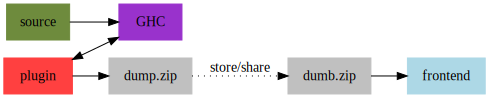
\includegraphics[width=0.8\textwidth]{figs/architecture.png}
  \caption{Dataflow diagram of the tool}
  \label{fig:architecture}
\end{figure}


% \digraph{abc}{
%   rankdir=LR
%     
%   source [label = "✍source",shape=MSquare, color="darkolivegreen4",style=filled]
% 
%   subgraph plugin {
%     style=filled;
%     color=lightgrey;
%     node [style=filled,color=gray,shape=box];
%     label = "plugin";
%     
%     ghc [label="🔨GHC",color="darkorchid"]
%     plugin [color="brown1",label="🧩plugin"]
%     dump1 [label = "📁dump.zip"]
%     dump2 [label = "📁dumb.zip"]
%   
%     source -> ghc
%     plugin -> ghc [dir=both]
%     plugin -> dump1
%     dump1 -> dump2 [style=dotted]
%   
%     dump2 -> frontend
%   }
% 
%   subgraph frontend {
%     node [style=filled];
%     label = "frontend";
%     color=blue
%     frontend [color=lightblue,label="🕵frontend"]
%   }
% }
% 
\section{Creating the GHC plugin}

The least invasive option would be to parse the output of GHC given a number of \mono{-ddump} flags. However, for the sake
of convenience and robustness, we instead decided to create a plugin that hook directly into the core2core pipeline and
capture the ASTs completely has original value. By interspersing each transformation with snapshot action we have as much information
as we could reasonably hope for.

\subsection{Capturing the information}
\label{section:methods:capturing_info}

If we wish to support multiple recent versions of GHC we need to deal with the fact that the Core ADT has undergone
a few minor changes and additions. We believe that the solution is to create some auxiliary definition to which we can
map various versions of the Core ADT. This was done very efficiently by building upon the existing \mono{ghc-dump} package,
which already implemented such a representation as well as a version agnostic conversion module with the help of \mono{min_version_GHC}
macro statements \cite{ghc_dump}. 

What \mono{ghc-dump} also intelligently addresses, is the issue of possible infinite recursion.
This problem arises through the \mono{IdInfo} struct attached to each variable such that the inliner
knows the body of variable when it wishes to inline the variable. However, when a variable represents a recursive ---
or even mutually recursive --- value, the inlining will contain itself. This fact implies that we can never serialise 
the AST to a finite value. Therefore, \mono{ghc-dump} demotes each usage site of a variable to an identifier referencing its binding site.
This allows us to obtaining a finite representation that we can later reconstruct by traversing
the AST with an environment.

\subsection{Globally unique variables}

It is not strictly necessary for variable names in a Core program to be unique. A variable name always
references the nearest binding site. However, is not very convenient
when we want to analyze a certain variable in isolation. After all, we cannot know if two separate free variables
with the same name are actually the same variable or live in a different scope. Consider the definition of tail:

\begin{listing}[H]
\begin{minted}[linenos]{haskell}
tail xs = case xs of
  x:xs -> xs
  _    -> error "tail of empty list"
\end{minted}
\end{listing}

We cannot simply refer to the variable \mono{xs} as that name has two different binding sites.
We solve this by running a \textit{uniquefication pass} as part of each snapshot that freshens all duplicate names in the entire
module after each core2core transformation. After this operations every variable is globally unique. 
This gives us the ability to refer to a binding site and its usages unambiguously using simply an identifying integer.
The big idea here is that any viewing logic is completely decoupled from binding semantics:

\begin{listing}[H]
\begin{minted}[linenos]{haskell}
tail xs_0 = case xs_0 of
  x_1:xs_2 -> xs_2
  _        -> error "tail of empty list"
\end{minted}
\end{listing}

It is possible to omit the numbered suffixes when displaying the AST, but internally it is very useful to be able to make
this distinction without any further effort.

\subsection{Detecting changes}

If a module is of a slightly larger size, it becomes difficult to spot the changes made by a certain
transformation, if there even are any. To address this, we decided to develop a feature that allows for
the filtering of code that remains unchanged. Let us define what unchanged means in this context. It is
important to make the subtle distinction between syntactic equivalence and $\alpha$-equivalence. The difference
is that the latter is agnostic to the names of variables, as long as they refer to the same binding site.

We can quickly solve the decision problem of syntactic equality by calculating a hash of an expression beforehand
and simply checking for equality of this hash value. We considered using recent improvements of full sub expression
matching \cite{hashing_mod_alpha}, but decided against it as it was not clear how to effectively present the results
nor did it rarely prove useful to isolate changes in the AST as they were rarely local to begin with.
Instead, we opted for a far simpler approach where we only hash the top-level definitions, and provide a more crude
option to hide any top-level definitions that have not changed at all.

All in all, we still recommend that issues are attempted to be reproduced in small modules as the amount of
noise can quickly become overwhelming despite change detection.

\section{Creating the frontend application}

We begin with a brief introduction to the Elm language and its concepts. Elm is very much a domain specific language; It is 
similar enough to Haskell to be familiar yet sufficiently simplified to be a frontend only language. It contrains the architecture
to a trinity of concepts.

\begin{itemize}
  \item \textbf{Model} - The state of the application
  \item \textbf{Update} - The way the state is updated: \mono{Message -> Model -> Model}
  \item \textbf{View} - The way the state is rendered: \mono{Model -> Html}
\end{itemize}

The big idea is to have exclusively \textit{pure} and \textit{complete} functions to handle viewing and updates.
These updates are triggered by so-called ``messages'' that are the result of user interaction like hovering, clicking, etc.
The increment/decrement example is a testament to the simplicity focused design of the language \cite{elm_lang}:

\begin{listing}[H]
\begin{minted}[linenos]{elm}
import Browser
import Html exposing (Html, button, div, text)
import Html.Events exposing (onClick)

main = Browser.sandbox { init = 0, update = update, view = view }

type Model = Int
type Msg = Increment | Decrement

update : Msg -> Model -> Model
update msg model =
  case msg of
    Increment -> model + 1
    Decrement -> model - 1

view : Model -> Html Msg
view model =
  div []
    [ button [ onClick Decrement ] [ text "-" ]
    , div [] [ text (String.fromInt model) ]
    , button [ onClick Increment ] [ text "+" ]
    ]
\end{minted}
\end{listing}

Unlike Haskell, the lack of explicit IO means that it feels justified to disallow any form of errors and by extent incomplete functions.
This powerful property gives us great confidence in the robustness of our application.

\subsection{Reproducing the AST}

It would have been extremely tedious to have to constantly maintain a Core ADT in Elm along with a JSON
parser that is compatible with the JSON output of the Haskell plugin. Luckily, we were able to use the
\mono{haskell-to-elm} \cite{haskell_to_elm} package to automatically derive all the required boilerplate code.

For example the \mono{Alt} datatype (i.e. an arm of a case expression) is defined as follows in our AST:

\begin{listing}[H]
\begin{minted}[linenos]{haskell}
data Alt = Alt
    { altCon :: AltCon
    , altBinders :: [Binder]
    , altRHS :: Expr
    }
    deriving (Generic)

deriving instance SOP.Generic Alt
deriving instance SOP.HasDatatypeInfo Alt
type AltElm = ElmType "Generated.Types.Alt" Alt
deriving via AltElm instance Aeson.ToJSON Alt
deriving via AltElm instance HasElmType Alt
deriving via AltElm instance HasElmDecoder Aeson.Value Alt
\end{minted}
\end{listing}

Note how we derive the \mono{Aeson.ToJSON} instance via the \mono{ElmType} machinery. This control allows
us to generate a compatible and robust JSON parser for Elm. The auto-generated Elm datatype and parser
(decoder in Elm speak) look like this:

\begin{listing}[H]
\begin{minted}[linenos]{elm}
type alias Alt =
    { altCon : AltCon
    , altBinders : List Binder
    , altRHS : Expr
    }

altDecoder : Json.Decode.Decoder Alt
altDecoder =
    Json.Decode.succeed Alt |>
    Json.Decode.Pipeline.required "altCon" altConDecoder |>
    Json.Decode.Pipeline.required "altBinders" (Json.Decode.list binderDecoder) |>
    Json.Decode.Pipeline.required "altRHS" exprDecoder
\end{minted}
\end{listing}

Conveniently, it would be very easy in the future to extend the Haskell ADT with additional information
because it is the single source of truth; The Elm type and JSON machinery can then be regenerated with a single command.

Additionally, we use this pipeline embellish the AST to allow for reconstruction of the demoted call sites (see \cref{section:methods:capturing_info}).
Specifically, we add a field to each \mono{BinderId} of the type:

\begin{listing}[H]
\begin{minted}[linenos]{haskell}
type BinderThunk = Found Binder | NotFound | Untouched
\end{minted}
\end{listing}

Initially this field is set to the \mono{Untouched} variant. Once the finitely encoded AST is decoded into the 
Elm universe, a reconstruction traversal takes place that, with the help of an environment, strengthens the 
\mono{BinderThunk} with a reference to its binder. The \mono{NotFound} variant exits purely for verification purposes
and should never occur with sound inputs. It is also important to note that Elm's single static assignment
semantics naturally implies that the \mono{Binder} is never copied, but only referenced.

After this initial reconstruct we again no longer need to keep binding semantics in mind, and we can isolate
subexpressions without explicit environments.

\subsection{Pretty printing}

It certainly should be considered useful to display the Core in exactly the same way that
GHC does. After all, this is what programmers are currently already used to and its design
has been given a lot of thought. However, we felt a need to first create a separate representation
that is tailored to those who have not seen Core before.

Haskell programmers that care enough to inspect the interaction with the compiler are likely to be
avid readers of at least basic Haskell syntax. Therefore, we decided to create a pretty printer that attempts
to be as similar to Haskell source as possible. Just like GHC, we used pretty printing the method developed 
by Wadler \cite{prettier_printer}, implemented in Elm using \mono{elm-pretty-printer} \cite{prettier_printer_elm}.
We believe that such a representation is a suitable way to minimize the shock reactions in newcomers, as well as
provide a more comfortable viewing experience for those who are primarily interested in the structure of their program
throughout optimisation.

To compare, consider again the Core representation presented in \cref{section:background:ghc} with the quicksort
representation produced by our pretty printer:

\begin{listing}[H]
\begin{minted}[linenos]{haskell}
quicksort :: forall a. Ord a -> [a] -> [a]
quicksort a $dOrd ds = case ds of
  { : x xs -> GHC.Base.++ @a
                (quicksort @a $dOrd
                   (GHC.List.filter @a
                      (\ds -> GHC.Classes.< @a $dOrd ds x) xs))
                (GHC.Base.++ @a
                   (GHC.Base.build @a
                      (\a c n -> c x n))
                   (quicksort @a $dOrd
                      (GHC.List.filter @a
                         (\ds -> GHC.Classes.> @a $dOrd ds x) xs)))
    [] -> GHC.Types.[] @a
  }
\end{minted}
\end{listing}

Notice that although this might look like normal Haskell, it contains explicit type variables like
\mono{a}, hinting at the SystemFC nature of Core. 

To facilitate syntax hightlighting, the pretty printer adds the appropriate token identifiers such that 
\mono{pygments} \cite{pygments} can be used to colorize the output.


\subsection{Including the source}
It goes without saying that the source code of a module is an essential part of any analysis. Therefore,
the plugin copies the source code and runs it through the \mono{pygmentize} \cite{pygments} tool to obtain
an HTML representation of the source code that is highlighted exactly the same way as the pretty printed Core.
This HTML source code is embedded in the output of the dump.

The artifacts produced by a single module now look like this:

\begin{listing}[H]
\begin{minted}[linenos]{text}
Quicksort_0.json
Quicksort_10.json
Quicksort_11.json
Quicksort_12.json
Quicksort_13.json
Quicksort_14.json
Quicksort_15.json
Quicksort_16.json
Quicksort_17.json
Quicksort_18.json
Quicksort_1.json
Quicksort_2.json
Quicksort_3.json
Quicksort_4.json
Quicksort_5.json
Quicksort_6.json
Quicksort_7.json
Quicksort_8.json
Quicksort_9.json
Quicksort.html
Quicksort_meta.json
\end{minted}
\end{listing}

All these files will be compressed in a zip archive to keep the size of the output smaller. It also makes for
a convenient atomic entity to load up in the frontend application where it is unzipped on the fly.

\subsection{Unfoldings and capture sizes}

As mentioned in \cref{section:methods:capturing_info}, the entire body of a variable is sometimes saved as part
of its \mono{IdInfo} which is exported to interface files such that inlining can take place across modules.
This part of the \mono{IdInfo} struct is called the \textit{unfolding} of a variable.
By nature, this can be a very large expression. At this time, we have no
need for the exact unfolding in the frontend application, other than knowing it exists. Therefore, we decided 
to replace any unfolding with a string literal to indicate that the unfolding was removed:

\begin{listing}[H]
\begin{minted}[linenos]{haskell}
removeUnfolding :: Unfolding -> Unfolding
removeUnfolding u@CoreUnfolding {..} = 
  u { unfTemplate = ELit (MachStr (T.pack "unfolding removed by plugin")) }
removeUnfolding x = x
\end{minted}
\end{listing}

This reduces the size of captures in some cases by a factor of 2.

\subsection{Interactions}

Aside from a more human-readable representation and syntax highlighting, the user is further supported by
a number of interactive features. These include:

\begin{itemize}
  \item Highlighting binding and call sites of a variable on hover
  \item Renaming variables
  \item Toggling various Core display options such as hiding typelevel terms and type applications, desugaring
        leading lambda abstractions, etc.
  \item Multiple approaches to hiding toplevel bindings such as hiding all but the selected binding, which
        can conveniently be followed up by un-hiding its referenced bindings transitively.
  \item A variable detail popup that shows all the available information of a variable.
  \item Querying variables and their types on Hoogle.
\end{itemize}

\subsection{Improving performance with cache semantics}

The way that Elm operates --- like many other interactive browser based applications --- is by rendering the HTML on every
update and then diffing the result with the current state of the DOM to create a minimal change list. This is generally a very
good strategy because mutating the DOM is by far the most dominant cost contributor. However, when it comes to pretty printing a
large Core expression the \mono{view} function starts to incur a significant cost. This is wasteful because many updates do not
actually affect the output of the pretty printer (events like \mono{onHover} and \mono{onClick} for example).
Initially this led to some serious usability issues where the application would stutter and freeze.

We were able to overcome this problem using the \mono{Html.Lazy} module. which takes some HTML producing closure and its arguments
separately. If on some update the arguments have not changed, the closure is not evaluated and a cached result is returned. Regardless,
the aforementioned diffing still takes place, reducing the cost of the update to something negligible. Of course, we cannot get around the fact that
any updates that do affect the output of the pretty printer might still cause some stutters, but the frequency of such updates is 
generally far lower.

\subsection{Note on deployment}

By virtue of being solely a stateless HTML + JavaScript application after compilation, means that the frontend can
easily and cheaply be deployed to any static file hosting service. Because the dump files are never send to the server,
we can discard any privacy concerns while still providing a no effort method to analyze the dumps. Anyone is still free
of course, to build and host their own build of the frontend which is similarly open sourced.


\newpage


\chapter{Results}

We discuss the results obtained using the tool through a number of real world cases.
The first of these additionally serves as a comprehensive, didactic, example of how to use the tool. 

\section{Diagnosing a failing inspection test in \mono{Text}}

Hearkening back to \mono{inspection-testing} discussed in \cref{section:introduction_inspection_testing}, we put
ourselves in the shoes of a programmer who gets surprised by a failing inspection test and reason how we might
employ HsComprehension to diagnose the problem. 

To summarize, we expected that the function \mono{countChars} which counts the number of characters in a \mono{ByteString}
using a number of functions in the \mono{Text} library, will in its final form not actually construct a \mono{Text} value.

\paragraph{1. Isolate the problem}
Modules typically contain more than 1 function and during the core2core transformations many more auxiliary functions are
added, and many functions are inlined to produce exponentially more code. Despite the tool being designed with features to 
comprehend medium-sized modules, it is still most helpful to temporarily isolate the
failing test case into a separate module:

\begin{minted}{haskell}
{-# LANGUAGE TemplateHaskell #-}

module InspectionTests where

import Test.Inspection
import qualified Data.Text as T
import qualified Data.Text.Encoding as TE
import Data.ByteString

countChars :: ByteString -> Int
countChars = T.length . T.toUpper . TE.decodeUtf8

-- the failing test case
inspect $ 'countChars `hasNoType` ''T.Text
\end{minted}

The following error is produced by the build:

\begin{minted}{sh}
app/InspectionTests.hs:21:1: countChars `hasNoType` Data.Text.Internal.Text failed:
# ...
# 700 lines of core as seen at the end of the core2core pipeline
# ...
\end{minted}

700 lines of textual data is generated from just this one function!
It is also incomplete in the sense that it does not show the process that produced this final
artifact.

\paragraph{2. Creating a capture}

Because we only want to create a capture of this module, we can use an exported TemplateHaskell primitive
that registers the plugin for the current module only by simply adding the \mono{dumpThisModule} snippet 
anywhere at the toplevel: 

\begin{listing}[H]
\begin{minted}{haskell}
{-# LANGUAGE TemplateHaskell #-}
import HsComprehension.Plugin (dumpThisModule)

...

dumpThisModule
\end{minted}
\end{listing}

Following a successful build, we can bundle the generated artifacts to a zip archive by running:

\begin{listing}[H]
\begin{minted}{sh}
$ cabal run hs-comprehension-zip
Attempting to archive dump files in ./dist-newstyle/coredump-Default
Archiving 23 files
Created /home/hugo/repos/hs-comprehension/test-project/dist-newstyle/Default.zip
\end{minted}
\end{listing}

\paragraph{3. Finding the root cause}
We navigate to \href{https://core.hugopeters.me}{core.hugopeters.me} and upload the zip archive we just
produced.

\begin{figure}[H]
\centering
\includegraphics[width=0.8\textwidth]{figs/countchars_1.png}
\label{fig:countchars_1}
\end{figure}

We then click the green arrow to reference the capture in the staging area. Here we could elect to stage more
than one capture if we want to compare them. In this case we are only interested in the current situation, and so we
just open a single panel tab with this single capture


\begin{figure}[H]
\centering
\includegraphics[width=0.8\textwidth]{figs/countchars_2.png}
\label{fig:countchars_2}
\end{figure}

On the left, are immediately presented with a number of viewing options. To the right we can see the rendered
Core, under influence of the view options. Above it a slider indicating that we are looking at the
Core in the desugared stage (so without any transformations yet applied). Scrolling this slider will reveal
the intermediate Core ASTs that were produced by the compiler. Whenever rewrite rules are fired they are included
as comments at the top of the module.

As you can see, the desugaring process has produced another top-level definition, namely \$\mono{trModule}. Since we
not care for anything but our \mono{countChars} function at this time, we can elect to filter out all other definitions,
including those that will be generated in the future: 

\begin{figure}[H]
\centering
\includegraphics[width=0.8\textwidth]{figs/countchars_hideallbut.png}
\label{fig:countchars_3}
\end{figure}

If we then scroll all the way to the end, we get the same final Core AST as we saw in the error message. Granted,
we now have syntax highlighting and a slightly more readable representation, but it is still unwieldy. Using a basic string search we can find the needle in the haystack:

\begin{figure}[H]
\centering
\includegraphics[width=0.8\textwidth]{figs/countchars_3.png}
\end{figure}

But we don't really care about finding the needle, but more so how it got it there.
Using the scroll bar we can go back in time to a moment before everything was inlined.
Specifically, we can go back to the first moment where no \mono{Text} constructor existed yet:

\begin{figure}[H]
\centering
\includegraphics[width=0.8\textwidth]{figs/countchars_4.png}
\end{figure}

We find a far more manageable definition of \mono{countChars} that has partially been transformed to operate on streams (\mono{Stream Char}).
This is a concept to faciliate fusion based on the work of D. Couts et al. \cite{stream_fusion}, we will discuss its theory more
in depth in next section. For now, it is only important to realise that instead of embedding the
incoming \mono{ByteString} in a \mono{Text} value, we are converting to a \mono{Stream Char} first before \mono{unstream}
converts to an actual \mono{Text}. The argument that this is not necessary still holds because there conceivably exists a length
function for values of type \mono{Stream Char} as well. 

So we can conclude that the \mono{text}'s fusion machinery did not produce the optimal result because it is conceivable to find the
length of a stream directly using some alternative \mono{length :: Stream Char -> Int} function.

\paragraph{4. Back to the future}

Luckily, we were reliving someone else's experience, and we have the luxury of seeing how the situation unfolded.
So, what we can do is make another capture with a more recent version of the library, and compare the two:

\begin{figure}[H]
\centering
\includegraphics[width=0.8\textwidth]{figs/countchars_5.png}
\end{figure}

Because we now have more than 1 capture open at the same time we can use the \textit{Hide common definitions} feature to
find the first moment where the two captures converge. This happens to be at phase 1 of the simplifier pass:

\begin{figure}[H]
\centering
\includegraphics[width=0.9\textwidth]{figs/countchars_6.png}
\end{figure}

For clarity, let us extract the text from both panels and compare them:

\begin{listing}[H]
\begin{minted}[linenos,fontsize=\footnotesize]{haskell}
{-
    Text-Bugged.zip
    RULES FIRED:
    STREAM stream/decodeUtf8 fusion (Data.Text.Encoding)
-}

countChars :: ByteString -> Int
countChars x = Data.Text.length
                 (Data.Text.Internal.Fusion.unstream
                    (Data.Text.Internal.Fusion.Common.toUpper
                       (Data.Text.Internal.Encoding.Fusion.streamUtf8 Data.Text.Encoding.Error.strictDecode x)))

------------------------------------------------------------------
{-
    Text-Patched.zip
    RULES FIRED:
    STREAM stream/decodeUtf8 fusion (Data.Text.Encoding)
    STREAM stream/unstream fusion (Data.Text.Internal.Fusion)
-}

countChars :: ByteString -> Int
countChars x = Data.Text.Internal.Fusion.length
                 (Data.Text.Internal.Fusion.Common.toUpper
                    (Data.Text.Internal.Encoding.Fusion.streamUtf8 Data.Text.Encoding.Error.strictDecode x))
\end{minted}
\end{listing}

The most notable difference is the extra rewrite rule that was fired in the patched version (line 18).
Unfortunately, it is currently not possible to look up the definition of the rewrite rule in the tool itself, but
given that we know its name and originating module, we can find it in the source of \mono{text} without too much effort:

\begin{listing}[H]
\begin{minted}{haskell}
{-# RULES "STREAM stream/unstream fusion" forall s. stream (unstream s) = s #-}
\end{minted}
\end{listing}

From this we learn that at some point there was a stream/unstream pair to remove. Another difference is the module from which
the \mono{length} function is imported (\mono{Data.Text.Internal.Fusion.length} over \mono{Data.Text.length}). Like we predicted earlier,
the patched version uses a variant that operates directly on streams:

\begin{figure}[H]
\centering
\includegraphics[width=0.8\textwidth]{figs/countchars_7.png}
\end{figure}

Given that in the previous in pass the captures were identical, and since no rewrite rule fired regarding \mono{length},
we can ascribe the difference to the inlining of \mono{length}. If we collect the definition of \mono{length} from both versions
of the text library we get:

\begin{listing}[H]
\begin{minted}{haskell}
-- Text-Bugged.zip
length :: Text -> Int
length t = S.length (stream t)
{-# INLINE [0] length #-}

-------------------------------------------

-- Text-Patched.zip
length :: Text -> Int
length t = S.length (stream t)
{-# INLINE [1] length #-}
\end{minted}
\end{listing}

The only difference is the phase annotation of the \mono{INLINE} pragma. The maintainers somehow decided that it was better
to inline \mono{length} one simplifier phase earlier (remember, phase 1 comes \textbf{before} phase 0). And they turned out to be right,
because inlining earlier uncovered the opportunity for the \textit{stream/unstream} rule to fire and remove 
the need to allocate an intermediate \mono{Text} value; Another exemplary manifestation of the Cascade Effect.

\paragraph{5. Epilogue: Brittleness of implicit fusion}
At or around the same time as Breitner. \cite{inspection_testing} identified the failed fusion case, Andrew Lelechenko had discovered
a problem involving the \mono{tail} function \cite{two_tails} under fusion. \mono{tail} just needs to drop the first character.
Despite needing to check whether to skip 1 or 2 bytes because of the UTF-16 encoding, this can be done in $O(1)$ time and memory.
Obviously this property should still hold when applying \mono{tail} twice in row. As it turns out, it does not. The following steps occur:

\begin{listing}[H]
\begin{minted}{haskell}
tail . tail
-- { inline to fusion variant }
unstream . S.tail . stream . unstream . S.tail . stream
-- { apply 'stream . unstream = id' }
unstream . S.tail . S.tail . stream
\end{minted}
\end{listing}

By constructing a stream we have become committed to traversing the entire structure where it was not needed at first,
yielding an $O(n)$ time and memory version after ``optimisation''. This is different from the situation in \mono{countChars},
where UTF-16 already dictated $O(n)$ runtime.

The ending to this story is quite simply that implicit fusion was disabled entirely \cite{two_tails} for similar functions.
Frequent \mono{text} contributor, Oleg Grenrus, remarked the following on the proposal to remove them:

\textit{``I think this is the right thing to do. Implicit fusion is unpredictable, and you explain, doesn't even work in simple cases.''}

Instead, users can now opt in by using the stream variant of such functions explicitly. This is a tragic example of how optimisation
can be unpredictable, and by extent, how people would favour predictability over automatic performance transformations that risk making the program slower.

\section{Lists vs Streams}

\begin{minted}{haskell}
Rec {
-- RHS size: {terms: 17, types: 17, coercions: 0, joins: 0/1}
Main.unlines [Occ=LoopBreaker]
  :: [GHC.Base.String] -> GHC.Base.String
[GblId, Arity=1, Str=<1L>, Unf=OtherCon []]
Main.unlines
  = \ (ds_s26z [Occ=Once1!] :: [[GHC.Types.Char]]) ->
      case ds_s26z of {
        [] -> GHC.Types.[] @GHC.Types.Char;
        : y_s26B [Occ=Once1] ys_s26C [Occ=Once1] ->
          let {
            sat_s26E [Occ=Once1, Dmd=ML] :: GHC.Base.String
            [LclId]
            sat_s26E = Main.unlines ys_s26C } in
          case GHC.Base.++ @GHC.Types.Char y_s26B Main.main5
          of sat_s26D [Occ=Once1]
          { __DEFAULT ->
          GHC.Base.++ @GHC.Types.Char sat_s26D sat_s26E
          }
      }
end Rec }

Rec {
-- RHS size: {terms: 17, types: 18, coercions: 0, joins: 0/1}
Main.unlines_go1 [Occ=LoopBreaker]
  :: [[GHC.Types.Char]] -> [GHC.Types.Char]
[GblId, Arity=1, Str=<1L>, Unf=OtherCon []]
Main.unlines_go1
  = \ (ds_s25d [Occ=Once1!] :: [[GHC.Types.Char]]) ->
      case ds_s25d of {
        [] -> GHC.Types.[] @GHC.Types.Char;
        : y_s25f [Occ=Once1] ys_s25g [Occ=Once1] ->
          let {
            sat_s25i [Occ=Once1, Dmd=ML] :: [GHC.Types.Char]
            [LclId]
            sat_s25i = Main.unlines_go1 ys_s25g } in
          case GHC.Base.++ @GHC.Types.Char y_s25f Main.main4
          of sat_s25h [Occ=Once1]
          { __DEFAULT ->
          GHC.Base.++ @GHC.Types.Char sat_s25h sat_s25i
          }
      }
end Rec }

\end{minted}




Here we discuss the basic of the stream paper, how it operates, why Haskell has not implemented it by favouring join points and
finally how the compilation pipeline treats these 2.

Perhaps repeat the unlines example from the background section.

\section{Erroneous program structure recovery in GHC fusion}
As part of our initial experiments to validate the tool, we decided to attempt to reproduce the shot-cut fusion of \mono{unlines} as presented
in the paper \cite{shortcut_fusion}. This serendipitously led to the discovery of a performance bug in GHC. Namely, the definition:

\begin{listing}[H]
\begin{minted}[linenos]{haskell}
unlines :: [String] -> String
unlines ls = concat (map (\l -> l ++ ['\n']) ls)
\end{minted}
\end{listing}

can be observed to be compiled to the following Core using our tool:

\begin{listing}[H]
\begin{minted}[linenos]{haskell}
cr_chr :: Char
cr_chr = C# '\n'

cr :: [Char]
cr = : cr_chr []

go1 :: [[Char]] -> [Char]
go1 ds = case ds of
  { : y ys -> ++
                (++ y cr)
                (go1 ys)
    [] -> []
  }

unlines :: [String] -> String
unlines ls = go1 ls
\end{minted}
\end{listing}

This definition is problematic because every line is first traversed to append a newline character and then again to append it to the rest of the line
yielding an $O(n^2)$ runtime, while we already know that an $O(n)$ runtime is possible. We can confirm that this version is indeed less performant by
benchmarking both \mono{unlines} and \mono{Prelude.unlines} on the first 73 lines of lorem ipsum:

\begin{listing}[H]
\begin{minted}{text}
benchmarking our_unlines
time                 127.9 μs   (125.0 μs .. 130.7 μs)
                     0.997 R²   (0.996 R² .. 0.998 R²)
mean                 126.6 μs   (124.6 μs .. 128.4 μs)
std dev              6.532 μs   (5.742 μs .. 7.504 μs)
variance introduced by outliers: 53% (severely inflated)

benchmarking prelude_unlines
time                 80.23 μs   (79.87 μs .. 80.53 μs)
                     1.000 R²   (0.999 R² .. 1.000 R²)
mean                 79.70 μs   (79.05 μs .. 80.13 μs)
std dev              1.858 μs   (1.088 μs .. 2.962 μs)
variance introduced by outliers: 20% (moderately inflated)
\end{minted}
\end{listing}

So it is clear that \mono{Prelude} has defined \mono{unlines} in a more efficient manner, but that does not take away the fact that any such
expression as our version of \mono{unlines} can reasonable expected to fuse in the most optimal manner. We investigate the reason for the suboptimal
fusion by using our tool. The tool reports that the following Core is desugared from the source:

\begin{listing}[H]
\begin{minted}[linenos]{haskell}
unlines :: [String] -> String
unlines ls = Data.Foldable.concat Data.Foldable.$fFoldable[]
               (GHC.Base.map
                  (\l -> GHC.Base.++ l
                           (GHC.Base.build
                              (\c n -> c
                                         (GHC.Types.C# '\n') n))) ls)
\end{minted}
\end{listing}

Here we can observe that the list literal \mono{['\n']} is already represented as a list producer function that is recognized nice with the short-cut fusion
rules. We can hypthesize in the near future \mono{map} and \mono{++} will be rewritten to their \textit{build/foldr} representation, making the fusion rule
applicable. After the first transformation, which is the also first pass of the simplifier, we get the following:

\begin{listing}[H]
\begin{minted}[linenos]{haskell}
unlines :: [String] -> String
unlines ls = GHC.Base.build
               (\c n -> GHC.Base.foldr
                          (GHC.Base.mapFB
                             (\x y -> GHC.Base.foldr c y x)
                             (\l -> GHC.Base.build
                                      (\c n -> GHC.Base.foldr c
                                                 (c
                                                    (GHC.Types.C# '\n') n) l))) n ls)
\end{minted}
\end{listing}

We can see how concat has been specialized and also rewritten, as well as \mono{++}. The result of \mono{map} however, is a bit more peculiar; contrary to what the paper
suggested at the time, we instead observe a call to some function \mono{mapFP}. The tool directly allows us to call upon Hoogle to find the definition of this function,
and the extensive documentation of the GHC Base library gives us some context:

\begin{listing}[H]
\begin{minted}[linenos]{haskell}
-- Note eta expanded
mapFB ::  (elt -> lst -> lst) -> (a -> elt) -> a -> lst -> lst
{-# INLINE [0] mapFB #-} -- See Note [Inline FB functions] in GHC.List
mapFB c f = \x ys -> c (f x) ys
\end{minted}
\end{listing}

\begin{listing}[H]
\begin{minted}[linenos]{text}
{- Note [The rules for map]
~~~~~~~~~~~~~~~~~~~~~~~~~~~
The rules for map work like this.

* Up to (but not including) phase 1, we use the "map" rule to
  rewrite all saturated applications of map with its build/fold
  form, hoping for fusion to happen.

  In phase 1 and 0, we switch off that rule, inline build, and
  switch on the "mapList" rule, which rewrites the foldr/mapFB
  thing back into plain map.

  It's important that these two rules aren't both active at once
  (along with build's unfolding) else we'd get an infinite loop
  in the rules.  Hence the activation control below.

* This same pattern is followed by many other functions:
  e.g. append, filter, iterate, repeat, etc. in GHC.List

  See also Note [Inline FB functions] in GHC.List

* The "mapFB" rule optimises compositions of map

* The "mapFB/id" rule gets rid of 'map id' calls.
  You might think that (mapFB c id) will turn into c simply
  when mapFB is inlined; but before that happens the "mapList"
  rule turns
     (foldr (mapFB (:) id) [] a
  back into
     map id
  Which is not very clever.

* Any similarity to the Functor laws for [] is expected.
-}

{-# RULES
"map"       [~1] forall f xs.   map f xs                = build (\c n -> foldr (mapFB c f) n xs)
"mapList"   [1]  forall f.      foldr (mapFB (:) f) []  = map f
"mapFB"     forall c f g.       mapFB (mapFB c f) g     = mapFB c (f.g)
"mapFB/id"  forall c.           mapFB c (\x -> x)       = c
  #-}
\end{minted}
\end{listing}

This documentation does not give us any insight yet into the role of the \mono{mapFB} function. Perhaps the note \mono{[Inline FB functions]} can provide
some more insight:

\begin{listing}[H]
\begin{minted}[linenos]{text}
Note [Inline FB functions]
~~~~~~~~~~~~~~~~~~~~~~~~~~

After fusion rules successfully fire, we are usually left with one or more calls
to list-producing functions abstracted over cons and nil. Here we call them
FB functions because their names usually end with 'FB'. It's a good idea to
inline FB functions because:

* They are higher-order functions and therefore benefits from inlining.

* When the final consumer is a left fold, inlining the FB functions is the only
  way to make arity expansion to happen. See Note [Left fold via right fold].

For this reason we mark all FB functions INLINE [0]. The [0] phase-specifier
ensures that calls to FB functions can be written back to the original form
when no fusion happens.

Without these inline pragmas, the loop in perf/should_run/T13001 won't be
allocation-free. Also see Trac #13001.
\end{minted}
\end{listing}

Here we find the answer to why \mono{mapFB} exists: ``\textit{alls to FB functions can be written back to the original form
when no fusion happens}''. It is desirable to retain the structure of the original map if it is not fused away. \mono{mapFB} enables does just that,
it exposes an initial opportunity to fuse but is reversible using the \textit{mapList} rule if no fusion happens. This has the convenient effect that 
compiled code can more closely represent the original source code on the hand, but on the other hand also limits code size.

Let's explore this further. If we always rewrite \mono{map} to  \mono{build (\c n -> foldr (\x r -> c (f x) r) n xs)}, then we lose some structure in the code.
Every loop will then generate a local, recursive loop. For example, take the function: \mono{addTwo = map (+1) . map (+1)}.

addTwo ds =
      case ds of
        [] -> []
        y : ys ->
          let xs = addTwo ys
              x = y+2
          in x:xs




addTwo1 x -> x+2

addTwo xs -> map addTwo1 xs



\begin{listing}[H]
\begin{minted}[linenos]{haskell}
\end{minted}
\end{listing}


% Trying to reach the same conclusion as https://github.com/haskell/text/issues/202 (recursing into the mentioned https://github.com/haskell/text/pull/348)

\section{Performance regression at Channable}

%https://github.com/haskell/text/issues/202
%https://github.com/haskell/text/pull/348
%
%Another performance regression: https://gitlab.haskell.org/ghc/ghc/-/issues/22207

\section{Comparison with existing tools}

\newpage

\chapter{Discussion \& Future work}

\section{Review of the tech stack}
\label{section:discussion:review}

Through extensive deriving and code generation, we have bridged the gap between the two programming languages in our tech-stack
rather seamlessly. Overcoming this issue has led us to go down that path before realizing other drawbacks.

Because we always envisioned a degree of intractability for exploring the dumps -- as that is the largest chunk of the value proposition --
the creation of dumps should be a light task and in order to work on the newest version of GHC, the plugin needs to have
a minimal dependency footprint. Initially we thought that serialising to JSON would a natural fit, however with the added requirement
of needing to match the generated decoder at the Elm site, the JSON deriving strategy was dependend on more than just \mono{aeson}.
Concretely, this means when working on the latest commit of GHC the odds are very high that the plugin won't work because the underlying
dependencies are not compatible yet. We ran into this issue when trying to patch \mono{unlines} in \cref{section:results:unlines} and were
forced to analyze the effect of our patches the old-fashioned way by sifting through the textual output of GHC like described in \cref{section:background:ghc}.

Furthermore, the need to serialise the infinite Core AST datatype at all turns out to be problematic. 
As described in \cref{section:methods:capturing_info}, to make the representation finite we need to address the
issue of self-referential unfoldings by replacing call sites with only references to binding sites. This is fundamentally
flawed because during our research we stumbled upon an inconvenient truth in the documentation of \mono{IdInfo}:

\begin{listing}[H]
\begin{minted}{text}
Two 'Id's may have different info even though they have the same
'Unique' (and are hence the same 'Id'); for example, one might lack
the properties attached to the other.
\end{minted}
\end{listing}

More research is needed as to when this issue crops up as relevant shortcoming, but needless to say it is a concerning flaw in the
basis of our approach.

It is not immediately obvious what alternatives there are. Ideally there is would no need to serialise at all by using a terminal application
itself written in Haskell (at the cost of some interactive features that the web offers). But is not at all obvious how to plug in this into the
compiler pipeline directly. Besides, comparing two different compiler runs is completely of the table in this approach. A Haskell terminal application could
still relax some of the dependency pressure by using a far more stable serialisation library that is less likely to break with unreleased GHC versions.

Considering that human inspection of code aligns more with the responsibilities of haskell language server than the compiler itself, the argument
could be made that \mono{hls} is the right place to implement inspection tools. Similarly however, the counterargument that this goes beyond
the scope of a language server is equally valid. 

The tragic reality is that for this tool to work on bleeding edge GHC versions, it has itself to be part of the GHC build system, which is not
realistic at this stage.

\section{Embedding information in the AST}
A fundamental problem with the current snapshot approach is the aggregation of multiple changes -- even multiple kinds of changes -- happening in between
each snapshot. It is simply impractical to try to recover the full story that connects one snapshot to the next. This leads one to wonder the possibilities
that would be unlocked if GHC embed information about the changes it has made directly in the AST. Consider for example a constructor that indicates
that its contained expression was the result of an inlining:

\begin{listing}[H]
\begin{minted}{haskell}
data Expr b = 
  ...
  | Inlined Expr InlineDetails
  ...
\end{minted}
\end{listing}

Obviously these added nodes could be omitted during normal compilation to not affect memory and performance. Less obvious however is how these extra
nodes would interfere with the transformations themselves that often rely on deep matching. Take for example detecting an opportunity for beta-reduction:

\begin{listing}[H]
\begin{minted}{haskell}
betaReduce :: Expr b -> Expr b
betaReduce (App (Lam b e) arg) = substExpr b arg e
betaReduce e = e
\end{minted}
\end{listing}

The following invocation to \mono{betaReduce} would not work as expected:

\begin{listing}[H]
\begin{minted}{haskell}
betaReduce (Inlined (App (Lam b e) arg) details) = Inlined (App (Lam b e) arg) details
\end{minted}
\end{listing}

A good robust solution to this is not obvious. Furthermore, we need to respect correctness invariant of these extra nodes. If we do for example make
an extra case for \mono{betaReduce}:

\begin{listing}[H]
\begin{minted}{haskell}
betaReduce (Inlined (App (Lam b e) arg) details) = Inlined (substExpr b arg e) details
\end{minted}
\end{listing}

Then one should wonder if the \mono{Inlined} tag is still entirely accurate. It might be more reasonable to have tags live for only 1 transformation
step and be erased before the next one starts. This still allows for transient information to be captured and used for analysis without affecting
the pipeline all that much. But of course, further research is needed.


\section{Printing Core like GHC}
\label{section:discussion:printing}

We have shown how an alternative Core printer is highly beneficial for newcomers and those interested in the syntactical structure of a program,
it does not take away from the fact the current Core printer has its place. After all, reading Core as if it was Haskell is not entirely
ingenuous. Take the complete ignorance towards showing which let bindings are join points for example, information that can be crucial to
the transformation that a program undergoes.

Simply summarized, it cannot be a complete tool without allowing to display the  Core in a way that is as close to the original 
GHC output as possible, but of course still with benefits of an interactive exploration frontend. A skeleton for this alternative
pretty printer has partially been implemented but finishing it is a matter of future work.

\section{Incomplete transformation pipeline coverage}

During our research we have mainly discovered and discussed Core-debugging scenarios that involved the general syntactical structure of the code.
For example, which functions are being called after rewrite rules and inlinings.
Although program structure analysis might in fact be the main constituent of most Core
debugging sessions, we have barely scratched the surface of other problems that need to be debugged in Core,
and by extent the suitability of our tool to do so. Examples here would be inadequately strong analysis results, preventing what would have been
a sound and desirable transformation. One such under discussed topic is the role that correctly identifying join points play.
More research is needed into the full spectrum of Core related problems and the information required to deal with them.

\section{Post Core factors}

Despite the idealistic design principle of the 3 stage compiler (\cref{section:background:core_lang}), where the Core transformation middle-section
is responsible for all optimisations, reality throws a spanner in the works. A number of critical optimisations are only possible on
a level closer to the hardware. Because of this, performance regressions cannot always be attributed to the Core pipeline. A real world, exemplary
encounter with this fact is a performance regression of \mono{alfred-margaret} \cite{alfred-margaret}, a Haskell implement of the \textit {Aho-Corasick}
string search algorithm. After updating from GHC 8.8.4 to GHC 8.10.7 a 10$\%$ performance regression was observed, which is rather significant.
After ruling out significant changes in the dependencies, it was noted that the used LLVM backend version 12 was not yet well-supported by the new GHC
version. That is, LLVM 9 incidentally yielded better performance.

There is simply no way to account for this in the Core pipeline. However, our tool could be extended to capture more extensive build information that
could then be diffed during inspection. Therefore, if a user establishes that the Core is not the culprit, he or she can still request to get a report of
all mutations in the build processes. This would include the LLVM version, the used C compiler, the linker, the assembler, etc. 
This way the tool can still provide some leads during performance regression analysis.

Lastly, information could be retrieved information from GHC's \textit{Spineless, Taggless, G-machine} (STG),
which converts the functional code to imperative form.
This process similarly takes care of some optimisations that were otherwise not possible in the Core pipeline.
Whether, and if so how, this telemetry can play a useful role in the tool is an avenue for future research.

\section{Fusion by rewrite rules}

As part of collecting Core related performance issues from the past, we made the observation that rewrite rules were the usual suspects, and often rightly so.
Especially rewrite rule based fusion, either within GHC itself or as part of custom library, come with many brittle interactions that cause failures
on specific cases are after small changes. This naturally begs the question if rewrite rules are a suitable method for implementing fusion. We believe
research is needed to evaluate the feasibility of fusion specific transformations that rely on, and interfere less, with the simplifier.

\newpage


\bibliographystyle{abbrv}
\bibliography{refs}

\appendix
\clearpage
\pagenumbering{roman}

\end{document}
